\chapter{Verfahren zur Metallbearbeitung und Grundlagen der Elektrotechnik}
\label{cha:Metallbearbeitung und Elektrotechnik}

\section{Aufgabenstellung}

Es sind die wichtigsten Grundlagen zur Metallbearbeitung zu erlernen. Dazu sollen zunächst händische Verfahren erlernt werden, um anschließend Methoden zur
 maschinellen Bearbeitung kennen zu lernen. Schwerpunkt in dieser Aufgabe besteht darin, Fertigungsverfahren aus dem Bereich Zerspannung, Umformung und Fügung 
 an Problemstellungen anzuwenden. Des Weiteren sollen Kenntnisse über die wichtigsten Eigenschaften verschiedener Metallarten erlernt werden. Außerdem ist es 
 wichtig, dass Vorschriften zum Arbeitsschutz eingehalten und stets mit bedacht behandelt werden. Ziel ist eine angeleitete, aber selbstständig durchgeführte 
 Lösung eines Problems, mithilfe der einzelnen Bearbeitungsverfahren. \\
Zudem sollen anschließend grundlegende Kenntnisse im Bereich Elektrotechnik erlernt werden. Dazu sollen Problemstellungen zunächst theoretisch erarbeitet 
werden, um diese dann Anhand kleinerer Versuchsaufbaue zu erläutern. Dies findet zunächst im Bereich Gleichstrom statt und soll dann zu Problemen und 
Verfahren im Drehstrombereich übergehen. Hier ist es von entscheidender Rolle, dass auch wichtige Regeln und Vorschriften zur Arbeitssicherheit erlernt und 
beachtet werden, um Arbeitsunfälle zu verhindern. Des Weiteren sollen Tätigkeiten und Vorgehensweisen eines Elektrikers geschult werden, um diese an 
Problemstellungen anzuwenden und ein zielorientiertes Arbeiten zu gewährleisten. 

\section{Praktischer Lösungsansatz}

In der Metallverarbeitung gibt es verschiedene Verfahren zur Herstellung eines Werkstückes. Diese Verfahren werden in Hauptgruppen zusammengefasst und 
unterscheiden sich in ihrer Eigenschaft, wie sie Rohmaterialien bearbeiten oder verändern. Eines dieser Verfahren ist das Trennen. Hierbei handelt es sich 
um ein spanendes Fertigungsverfahren.
\begin{description}
\item[Spanende Fertigung] Die spanende Fertigung beschreibt ein Verfahren zur Bearbeitung verschiedener Werkstoffe mit Hilfe von Werkzeugen, bei denen 
Material vom Werkstoff herausgeschnitten wird, um dessen Form oder Oberfläche zu verändern. Das abgetragene Material wird auch als Span bezeichnet. %cite 1
\end{description}
Zu den spanenden Fertigungsverfahren zählen \zB das Feilen, Schleifen, Sägen, Bohren, Drehen und Fräsen. Jedes dieser Verfahren hat seine eigenen 
Eigenschaften und bietet sowohl Vor- als auch Nachteile. 
\paragraph{Feilen}\mbox{}\\
Das Feilen wird meist von Hand ausgeführt, mit sogenannten Werkstattfeilen und dient zur präzisen Bearbeitung von Werkstücken. Dies hat zur Folge, dass nur 
kleinere Arbeiten mit der Feile getätigt werden können, da andernfalls dieses Verfahren zu zeitaufwendig wäre. Im Gegensatz zur maschinellen Bearbeitung, 
wie \zB beim Fräsen oder Drehen, bietet dass Feilen den großen Vorteil, dass auch filigrane Arbeiten auf engem Raum getätigt werden können. Zudem 
unterscheiden sich Feilen in ihrer Bezahnung, auch Hieb genannt. Es gibt Feilen mit wenigen Hieben, welche ihren Anwendungsbereich in der Bearbeitung 
von weichen Werkstoffen wie Aluminium haben, aber auch zur Grobbearbeitung genutzt werden, um möglichst viel Material abzutragen. Feilen mit einer großen 
Anzahl von Hieben tragen nur wenig Material ab und sind meist ungeeignet für weiche Werkstoffe, da die Späne in den Zwischenräumen stecken bleiben, dafür 
erzeugen diese meist eine glatte Oberfläche mit einer höheren Güte. %cite 2
\paragraph{Fräsen und Drehen}\mbox{}\\
Das Fräsen ist neben dem Drehen eines der wichtigsten Verarbeitungsverfahren zur Bearbeitung von Werkstoffen. Beide Verfahren unterscheiden sich in den 
Anwendungsbereichen und wie sie die Werkstücke bearbeiten. Hierbei sind Werkstücke, die gedreht werden immer symmetrisch, da ausschließlich Runde 
Werkstoffe verarbeitet werden können. Dies liegt daran, dass beim Drehen sich das Werkstück um die eigene Achse dreht und beim Fräsen das Werkzeug. 
Durch diesen Unterschied hat jedes der beiden Fertigungsverfahren seinen eigenen Anwendungsbereich. Das Drehen wird \zB bei Bolzen, Schrauben oder 
Unterlagscheiben angewandt und das Fräsen bei \zB Nuten, Formänderungen oder Bohrungen. Heutzutage unterscheidet man zwischen zwei Arten des Fräsens 
und Drehens, dem konventionellen und dem Computerized Numerical Control (CNC) Fräsen oder Drehen. Beide Verfahren bieten einen sehr hohen Grad an Genauigkeit 
und finden einen großen Anwendungsbereich in der Fertigung präziser Werkstücke. Das Fräsen oder Drehen bringt den großen Vorteil mit sich, dass viel Material 
abgetragen werden kann und die Qualität darunter nicht in Mitleidenschaft gezogen wird. Durch die CNC Technologie ist das Fertigen gleichaussehender Teile 
automatisiert und für den Fließbandbetrieb ideal. Somit bietet dies Unternehmen die Chance Kosten durch schnelle und präzise Fertigung zu reduzieren. 
Allerdings gibt es auch Nachteile beim Fräsen oder Drehen, welche vor allem im thermodynamischen Segment liegen, da die Werkstoffe und Werkzeuge sehr 
großer Hitze ausgesetzt sind und somit die Gefahr herrscht, dass sich die Eigenschaften \zB des Metalls negativ verändern. Um diese thermische Belastung 
einzuschränken, werden oftmals Kühlflüssigkeiten verwendet, welche bei Kontakt eine Belastung für die Umwelt und Gesundheit darstellen. %cite 3
Ein weiteres Verfahren zur Bearbeitung von Werkstoffen, ist die Umformung. Der große Unterschied zu spanenden Fertigungsverfahren ist hierbei, dass kein 
Material entfernt wird. Es wird lediglich die Geometrie verändert, um die gewünschte Form zu erreichen. Da die meisten Metalle die Eigenschaft einer guten 
Verformbarkeit haben, wird dieses Verfahren überwiegend in der Metallindustrie verwendet. Zu solchen Verfahren zählen \zB Walzen, Schmieden und Biegen. Wobei 
in den meisten Unternehmen das Biegen eine größere Rolle spielt, da es einfach in der Anwendung und relativ kostengünstig ist. Beispielsweise könnte mit einem 
Stück Flachstahl ein Winkel erzeugt werden, um etwas zu befestigen. Ein klarer Vorteil kristallisiert sich dabei schnell heraus und zeigt, dass dieses 
Verfahren sehr einfach in der Anwendung und flexibel einsetzbar ist. Allerdings beschränkt sich dies sehr schnell auf einfache Problemstellungen, denn 
sobald ein komplexes Werkstück benötigt wird, reicht dieses Verfahren nicht mehr aus. Ein großer Nachteil ist beim Biegen, dass man einen Mindestbiegeradius 
einhalten sollte, da sich das Material sonst verjüngt oder gar bricht.
\begin{description}
\item[verjüngen] Begriff in der Technik für die Verringerung von Querschnitten im Material
\end{description}
Um dieses Verhalten zu unterbinden, sollte der Biegeradius vor Beginn der Arbeit beachtet werden. Dazu muss je nach Metallart ein Radius von ein oder zweimal 
der Stärke des Metalls genommen werden.\\
Das letzte wichtige Verfahren ist das Fügen. Hierbei werden zwei oder mehrere Werkstücke so verbunden, dass sie miteinander eine dauerhafte Verbindung 
erzeugen. Zu den wichtigsten Fügeverfahren zählt das Schweißen, welches in Unternehmen einen großen Anwendungsbereich findet. Sei es in der Verbindung 
und dem Bau von Rohren oder Schiffen, als auch in der Lösung von schnellen Problemen vor Ort, wie \zB zur Reparatur von Beschädigungen. Jeder Einsatzbereich 
hat andere Anforderungen an das Schweißen, was eine Vielfalt an Schweißmethoden und Verfahren voraussetzt. Eines dieser Verfahren ist das 
Lichtbogenhandschweißen, in dem mit Hilfe elektrischen Stroms ein Lichtbogen erzeugt wird, der die Materialien schmilzt und bei anschließender 
Aushärtung miteinander verbindet. Dieses sogenannte Schmelzbad muss durch Zufuhr von einem geeigneten Schutzgas, meist Argon umhüllt sein, um eine Oxidation 
mit dem Umgebungssauerstoff zu verhindern. Diese Oxidation würde zu einer Verschlechterung der Qualität und zu einer spröden Schweißnaht führen, was zur 
Folge hätte, dass diese nicht belastungsfähig wäre. Die Verwendung von Schutzgas wird nur in den Methoden des Metall-Inertgas- (MIG), Metall-Aktivgas- (MAG) 
und Wolfram-Inertgas-Schweißens (WIG) verwendet, da es bei diesen Methoden keine andere Möglichkeit zum Schutz des Schmelzbades gibt. Diese drei Methoden 
bieten den großen Vorteil einer hohen Produktivität, wie auch eine gute Automatisierung, da der Schweißdraht von einer Trommel automatisch und kontinuierlich 
zugeführt wird. Im Gegensatz zu diesen Methoden steht das Elektrohandschweißen mit einer Stabelektrode. Hierbei wird kein Schutzgas benötigt, da sich das 
Schweißbad durch die entstehende Schlacke und den Rauch selber vom Umgebungssauerstoff isoliert. Dies bietet dem Anwender den großen Vorteil, dass diese 
Methode nahezu überall anwendbar ist und keine großen Geräte mit Schutzgaszufuhr benötigen. Deshalb wird diese Methode auch häufig bei Problemstellungen 
im Außenbereich angewandt. Der größte Nachteil ist hierbei die hohe Rauchentwicklung, wie auch der entstehende Aufwand und Dreck bei entfernen der Schlacke. 
Hierzu sollte in geschlossenen Räumen immer eine Absaugung gewährleistet sein, da die Dämpfe gesundheitliche Folgen haben und nicht in großen Mengen 
eingeatmet werden dürfen. Zudem ist es beim Schweißen allgemein von hoher Relevanz, dass ein Augenschutz, wie auch eine geeignete persönliche 
Schutzausrüstung (PSA) getragen wird, um sich vor Funken und Strahlung durch den Lichtbogen zu schützen. \\\\ %\cite 4
Im Folgenden geht es um die Lösung von Problemen im Bereich Elektrotechnik. Hierzu wird sich der erste Teil auf die Lösung von Gleichstromproblemen und der 
zweite Teil auf die Lösung von Wechsel- oder Drehstromproblemen beziehen. Um einfache Gleichstromkreise zu berechnen, ist es von entscheidender Relevanz, 
die richtigen Formeln anzuwenden. Dazu gibt es \zB Formeln für Parallel oder in Reihe geschaltete Widerstände, die Kirchhoffschen Gesetze oder das ohmsche 
Gesetz. Alle diese Formeln dienen dazu, dass Verhalten von Widerständen zu beschreiben, um daraus praktische Schlüsse in der Anwendung dieser zu ziehen. 
Ein Widerstand hat unter anderem den Nutzen, die Spannung oder den Strom zu verringern, um den Verbraucher zu schützen. Je nachdem, welches Problem zu 
lösen ist, muss der Widerstand parallel, in Reihe oder beides in Kombination verwendet werden. Da es allerdings nur festgelegte Widerstandgrößen zu kaufen 
gibt und meist auch nicht alle im Unternehmen vorhanden sind, müssen verschiedene Größen miteinander kombiniert werden. Durch die Verwendung der Formel für 
parallelgeschaltete Widerstände, kann man \zB durch die Verwendung zweier 100 $\Omega$ Widerstände herausfinden, dass dadurch ein 50 $\Omega$ Widerstand 
entsteht. Dies kann beliebig oft angewandt werden, wobei die Formel 1.1 zur Berechnung von parallelen Widerständen nur für eine maximale Anzahl von zwei 
Widerständen und die Formel 1.2 für eine unbegrenzte Anzahl von Wideständen zählt.
\begin{equation}
R_{ges}=\frac{R_1*R_2}{R_1+R_2}
\label{eqn:Parallelschaltung von 2 Widerständen}
\end{equation}
\begin{equation}
\frac{1}{R_{ges}}=\frac{1}{R_1}+\frac{1}{R_2}+…
\label{eqn:Parallelschaltung von mehreren Widerständen}
\end{equation}
Zudem ist bei parallelgeschalteten Widerständen zu beachten, dass die Spannung, welche über den Widerständen abfällt immer gleich bleibt und diese Art der 
Verschaltung nur zu einer Reduktion des Stroms führt. Um den gesamten Strom über den Widerständen zu berechnen, kann folgende Formel angewandt werden.
\begin{equation}
I_{ges} = \frac{U}{R_{ges}}
\label{eqn:Gesamtstrom Parallelschaltung}
\end{equation}
Bei einer Reihenschaltung von Widerständen ist die Berechnung deutlich einfacher, da sich diese lediglich addieren. Somit können beliebig viele Widerstände in Reihe geschaltet werden, um den gesamten Widerstand zu erhöhen.
\begin{equation}
R_{ges}=R_1+R_2+…
\label{eqn:Widerstand Reihenschaltung}
\end{equation}
Allerdings ist bei einer Reihenschaltung zu beachten, dass eine Reduktion der Spannung über den Widerständen stattfindet, weshalb dieser Typ Verschaltung 
angewandt wird bei Verbrauchern, die eine geringere Spannung benötigen, als die anliegende. Zudem ist es möglich beide Typen der Verschaltung zu kombinieren. 
Hierbei ist dann jeweils zu beachten, welche der Formeln angewandt werden muss, da beide Typen vorhanden sind. Wichtig dabei zu beachten ist, dass das 
Schaltbild in einzelnen Teilschritten berechnet wird und man die beiden Formeln für die Reihen- und Parallelschaltung nicht vermischt. 
Allgemein gilt immer, dass man von innen nach außen rechnet und versucht am Ende auf einen Widerstand zu kommen, über dem die Spannung oder der Strom abfällt.
\clearpage
Im folgenden Beispiel wird eine solche Schaltung nochmals genauer erläutert.
\begin{figure}[hbt]
    \centering
    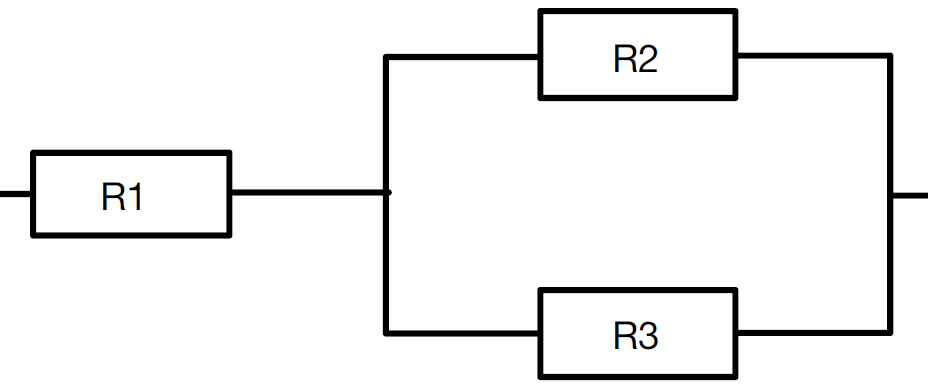
\includegraphics[width=0.8\linewidth]{images/Gemischte Schaltung}
    \caption[Gemischte Schaltung]{Gemischte Schaltung}
    \label{fig:Gemischte Schaltung}
\end{figure}
Hier ist es wichtig zuerst die Parallelschaltung zwischen $R_2$ und $R_3$ zu berechnen, um einen Gesamtwiderstand zu bekommen. Mit Hilfe dieses 
Gesamtwiderstandes kann nun die Reihenschaltung zwischen $R_{2,3}$ und $R_1$ berechnet werden. Schließlich kommt ein Widerstand für die gesamte Schaltung
heraus, über dem die angelegte Spannung abfällt.\\
Eine weitere wichtige Formel zur Berechnung von Gleichstromkreisen, ist die Knotenregel. Diese findet sich auch im 1. Kirchhoffschen Gesetz wieder und sagt 
aus, dass an jedem Knotenpunkt in einem Stromnetz gleichviele Ströme hinein-, als auch wieder hinausfließen. So kann an jedem Knotenpunkt, welcher nicht 
die gleichen Ströme wie ein anderer Knoten hat, eine Knotengleichung aufgestellt werden. Mit Hilfe dieser Gleichungen lässt sich anschließend ein 
Gleichungssystem lösen, was zur Lösung des Problems führen kann.
\begin{equation}
I_1+I_2+I_3=I_4+I_5
\label{eqn:1. Kirchhoffsches Gesetz}
\end{equation}
Gibt es allerdings noch eine unbekannte Variable, dann kann die Schaltung nicht alleinig mit der Knotenregel berechnet werden, sondern benötigt zusätzlich die 
Anwendung des 2. Kirchhoffschen Gesetzes, der Maschenregel. Diese Regel besagt, dass alle Spannungen in einer Masche, heißt in einem geschlossenen Stromkreis 
von Widerständen, Spannungsquellen, etc. in Summe Null ergeben. In Kombination mit der Knotenregel kann nun fast jedes einfachere Problem in einem 
Gleichstromkreis gelöst werden.
\begin{equation}
U_1+U_2+U_3-U_4-U_5=0
\label{eqn:2. Kirchhoffsches Gesetz}
\end{equation}
Dieses Verhalten von Widerständen in Bezug auf Strom und Spannung kann durch einfache Versuche nachgewiesen werden. Einer dieser Versuche wäre \zB, dass 
man einen einfachen Stromkreis aufbaut, der einen Widerstand und einen Verbraucher \zB eine Glühbirne beinhaltet. Variiert man nun mit der Größe des 
Widerstandes, kann man bei gleichbleibender Spannung feststellen, dass die Glühbirne dunkler wird, je größer der Widerstand wird.\\ 
Ein weiterer Versuch kann durchgeführt werden, indem man zwei Glühbirnen beim ersten Durchgang in Reihe schaltet und beim zweiten Durchgang 
parallelschaltet. Man wird beobachten, dass die Glühbirnen bei der Parallelschaltung heller leuchten, als bei der Reihenschaltung. Dies liegt daran, 
dass in der Reihenschaltung Spannung über der ersten Glühbirne abfällt, da diese einen Widerstand im Stromnetz darstellt. Somit liegt an der zweiten 
Glühbirne eine geringere Spannung an und Folge dessen leuchtet diese weniger. Bei einer Parallelschaltung ist dies nicht der Fall, da dort an jeder 
Glühbirne gleichviel Spannung anliegt. Es sinkt lediglich der Strom an jeder Glühbirne. 

\section{Reflexion und Bewertung}

Hier Text ...

\clearpage